%=========================================================================
% (c) 2011, 2012 Josef Lusticky

\section{Algorithms}\label{sec:ntp-algorithms}
Because of network latency the received Transmit Timestamp will never be exactly
corresponding to the current time.
One of the main goals of NTP is to deal with the network latency~\cite{ntp-overview}.

As described in section~\ref{sec:ntp-network},
there are the following 64-bit long timestamps in NTP packet: Origin, Receive and Transmit Timestamp.
Upon NTP packet arrival, the client determines another timestamp called
Destination Timestamp~\cite{rfc5905}.
This timestamp is represented as T4 in figure~\ref{fig:ntp-client-server}
and is not part of NTP packet structure.

Using these four timestamps, NTP client using unicast communication mode can compute
the local clock offset which is given by $\theta = \frac{1}{2}[(t_2 - t_1) + (t_3 - t_4)]$,
where $t_1$ is the time of the request packet transmission (Origin Timestamp),
$t_2$ is the time of the request packet reception (Receive Timestamp),
$t_3$ is the time of the response packet transmission (Transmit Timestamp) and
$t_4$ is the time of the response packet reception (Destination Timestamp)~\cite{ntp-algor,rfc5905}.
The implicit assumption in the above is that one-way delay is
statistically half of round-trip delay~\cite{rfc5905},
which is given by $\delta = (t_4 - t_1) - (t_3 - t_2)$.

In broadcast communication mode, Origin and Receive Timestamps are not accounted.
The client computes its local clock offset which is given by $\theta = t_3 - t_4$.
The implicit assumption in the above is that one-way delay from server to client is zero.
Since this is never the case, it is useful to provide an
initial volley where the client exchanges several packets with the server in
order to calibrate the propagation delay~\cite{rfc5905}.

When computing the result from more servers, the intersection algorithm is used
for selecting the possible most exact timestamp received from various servers~\cite{ntp-improved-algor,rfc5905}.
Intersection algorithm is derived from Marzullo algorithm but the basic
computation remains the same~\cite{ntp-history}.
First of all a selection of bad and good servers must be made.
Bad servers are called Falsetickers and good are called Truechimers~\cite{rfc5905}.
The division to these sets is based on their response.
As one can assume for a sensible result there must be more Truechimers than Falsetickers~\cite{rfc5905}.

After selecting a set of reliable servers, NTP clock algorithms compute resulting exact timestamp.
The resulting exact timestamp does not have to be the same
as one of those provided by the servers.
NTP clock algorithms calculate using clock accuracy estimates
determined from Root Dispersion, Root Delay and Precision fields of server's response.
These estimates are converted to intervals.
Figure~\ref{fig:ntp-intersection} shows the computation for the following example:
If we have the estimates $10 \pm 2$, $12 \pm 1$ and $11 \pm 1$
then these intervals are $<8; 12>$, $<11; 13>$ and $<10; 12>$ which
intersect to form $<11; 12>$ or $11.5 \pm 0.5$ as consistent with all three values.
The arithmetic mean is used as the result value.
When querying servers again, the algorithm repeats but the new result computation
also depends on the previous result~\cite{rfc5905,ntp-history}.
This eliminates possible jitter which can be caused by repeatedly querying the servers
and getting slightly different answers from them.

\begin{figure}
	\centering
	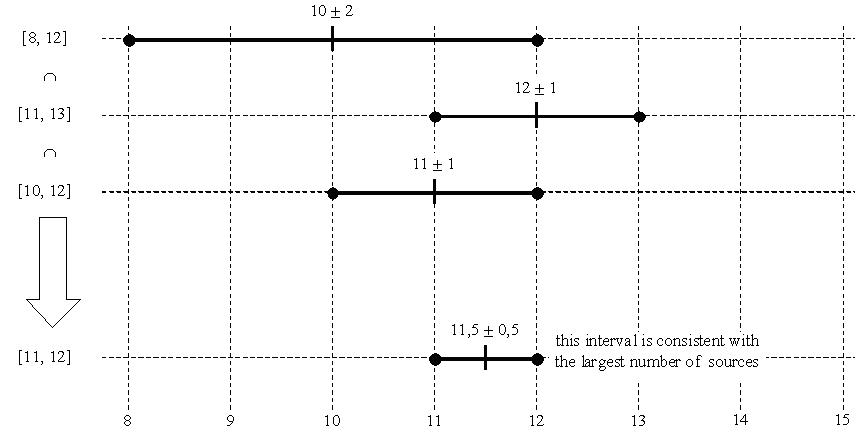
\includegraphics[width=13cm,keepaspectratio]{fig/Marzullo_example-1.jpg}
	\caption{Intersection algorithm (source:~\cite{wikipedia-marzullo})}
	\label{fig:ntp-intersection}
	\bigskip
\end{figure}

%Since the clients complying with a subset of NTP, called
%the Simple Network Time Protocol (SNTPv4) [RFC4330], do not need to
%implement the mitigation algorithms ... ~\cite{rfc5905}.
